\documentclass[11pt]{article}
 
\usepackage[text={6in,8.1in},centering]{geometry}

\usepackage{enumerate}
\usepackage{amsmath,amsthm,amssymb}
\usepackage{mathrsfs} % to use mathscr fonts

\usepackage{pstricks}
\usepackage{pst-solides3d}
\usepackage{pstricks-add}
\usepackage{graphicx}
\usepackage{pst-tree}
\usepackage{pst-poly}
\usepackage{calc,ifthen}
\usepackage{float}\usepackage{multicol}
\usepackage{multirow}
\usepackage{array}
\usepackage{longtable}
\usepackage{tikz}
\usepackage{tkz-berge}
\usepackage{fancyhdr}
\usepackage{algorithmicx,algpseudocode}
\usepackage{changepage}
\usepackage{color}
\usepackage{listings}
\usepackage{fancyvrb}

\lstset{ %
language=C++,                % choose the language of the code
basicstyle=\footnotesize,       % the size of the fonts that are used for the code
numbers=none,                   % where to put the line-numbers
numberstyle=\footnotesize,      % the size of the fonts that are used for the line-numbers
stepnumber=1,                   % the step between two line-numbers. If it is 1 each line will be numbered
numbersep=5pt,                  % how far the line-numbers are from the code
backgroundcolor=\color{white},  % choose the background color. You must add \usepackage{color}
showspaces=false,               % show spaces adding particular underscores
showstringspaces=false,         % underline spaces within strings
showtabs=false,                 % show tabs within strings adding particular underscores
frame=none,           % adds a frame around the code
tabsize=2,          % sets default tabsize to 2 spaces
captionpos=b,           % sets the caption-position to bottom
breaklines=true,        % sets automatic line breaking
breakatwhitespace=false,    % sets if automatic breaks should only happen at whitespace
escapeinside={\%*}          % if you want to add a comment within your code
}

\newenvironment{block}{\begin{adjustwidth}{1.5cm}{1.5cm}\noindent}{\end{adjustwidth}}

\newtheorem{proposition}{Proposition}[section]
\newtheorem{theorem}{Theorem}[section]
\newtheorem{lemma}{Lemma}[section]
\newtheorem{corollary}{Corollary}[section]
\theoremstyle{definition}
\newtheorem{definition}{Definition}[section]

\title{Extremal Functions on Cayley Digraphs of\\ Finite Cyclic Groups\footnote{Supported in part by National Science Foundation (NSF).}}
\author{{\sc Jordan Blocher}\\ 
Department of Mathematics\\ 
University of Nevada-Reno\\ 
Reno, Nevada, USA\\
{\tt jordanblocher@gmail.com}
\and 
{\sc Samantha Hampton}\\
Department of Mathematics\\
University of Arkansas\\
Fayetteville, Arkansas, USA\\
{\tt smhampto@uark.edu}
\and 
{\sc Christopher Linden}\\
Department of Mathematics\\
University of California  at Los Angeles\\
Los Angeles, California, USA\\
{\tt lindenechris@gmail.com} }
\date{\today}
 
 
\def\R{\mbox{$\mathbb R$}}
\def\Q{\mbox{$\mathbb Q$}}
\def\Z{\mbox{$\mathbb Z$}}
\def\N{\mbox{$\mathbb N$}}
\def\C{\mbox{$\mathbb C$}}
\def\Sym{\operatorname{Sym}}
\def\lcm{\operatorname{lcm}}
\def\adj{\operatorname{adj}}
\def\inc{\operatorname{inc}}
\def\Cay{\operatorname{Cay}}
\def\Geom{\operatorname{\cal G}}
\def\ker{\operatorname{ker}}
\def\kernel{\operatorname{ker}}
\def\automorphism{\operatorname{Aut}}
\def\endomorphism{\operatorname{End}}
\def\inner{\operatorname{Inn}}
\def\outer{\operatorname{Out}}
\def\crossing{\operatorname{cr}}
\def\cent{\textcent}
\def\n{\\ \vspace{1.7mm}}
\def\diam{\operatorname{diam}}

\renewcommand{\emptyset}{\O}
 
 
\newcounter{ZZZ}
\newcounter{XXX}
\newcounter{XX}
 
\headsep25pt\headheight20pt
 
 
\pagestyle{fancyplain}
\lhead{\fancyplain{}{\small\bfseries Blocher, Hampton, Linden,\ \ Cayley Digraphs of Finite Cyclic Groups}}
\rhead{\fancyplain{}{\small\bfseries\thepage}}
\cfoot{\ \hfill\tiny\sl Draft printed on \today}
 
 
\setlength{\extrarowheight}{2.5pt} % defines the extra space in tables
 
 
 
\begin{document}
 
\baselineskip6mm\parskip4mm

\maketitle
\begin{center}
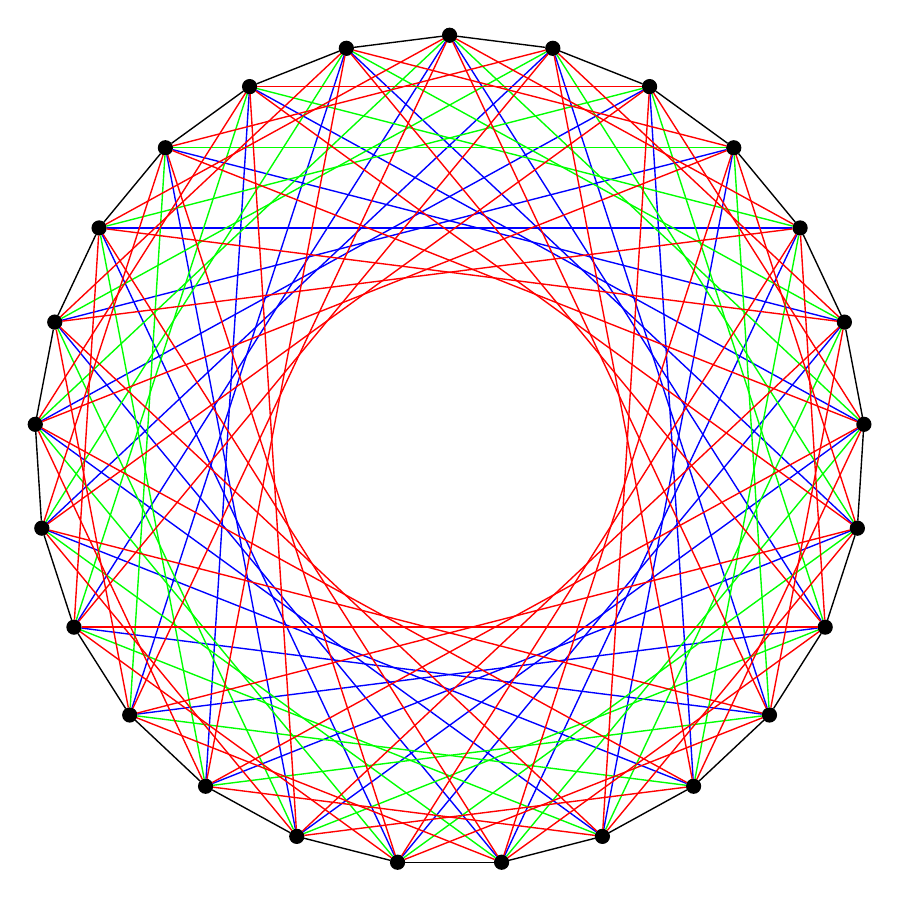
\begin{tikzpicture}


\GraphInit[vstyle=Simple]
\tikzset{VertexStyle/.append style = {minimum size = 5pt, inner sep = 0pt}}

\Vertex[x=187.5pt,y=337.5pt]{0};
\Vertex[x=224.80348307472823pt,y=332.7874741692947pt]{1};
\Vertex[x=259.7630511152573pt,y=318.94600200657953pt]{2};
\Vertex[x=290.1820658893033pt,y=296.8452941132117pt]{3};
\Vertex[x=314.14918882530225pt,y=267.87401924684946pt]{4};
\Vertex[x=330.15847744427305pt,y=233.85254915624213pt]{5};
\Vertex[x=337.2040092642407pt,y=196.91857792939703pt]{6};
\Vertex[x=334.8430876093033pt,y=159.3928028121413pt]{7};
\Vertex[x=323.22405786990294pt,y=123.63310626523908pt]{8};
\Vertex[x=303.0769864163684pt,y=91.88640153769651pt]{9};
\Vertex[x=275.667787843871pt,y=66.14745084375791pt]{10};
\Vertex[x=242.71868290270174pt,y=48.0335271167623pt]{11};
\Vertex[x=206.2999850346457pt,y=38.682794802828326pt]{12};
\Vertex[x=168.70001496535434pt,y=38.682794802828326pt]{13};
\Vertex[x=132.2813170972983pt,y=48.03352711676226pt]{14};
\Vertex[x=99.3322121561291pt,y=66.14745084375782pt]{15};
\Vertex[x=71.92301358363159pt,y=91.88640153769656pt]{16};
\Vertex[x=51.77594213009703pt,y=123.63310626523916pt]{17};
\Vertex[x=40.1569123906967pt,y=159.3928028121413pt]{18};
\Vertex[x=37.795990735759275pt,y=196.91857792939695pt]{19};
\Vertex[x=44.841522555726954pt,y=233.8525491562421pt]{20};
\Vertex[x=60.85081117469775pt,y=267.8740192468495pt]{21};
\Vertex[x=84.81793411069665pt,y=296.8452941132117pt]{22};
\Vertex[x=115.23694888474257pt,y=318.9460020065795pt]{23};
\Vertex[x=150.1965169252717pt,y=332.7874741692946pt]{24};

\SetUpEdge[lw         = .5pt,
            color      = black,
            labelcolor = black]

\Edge(24)(0)
\Edge(0)(1)
\Edge(1)(2)
\Edge(2)(3)
\Edge(3)(4)
\Edge(4)(5)
\Edge(5)(6)
\Edge(6)(7)
\Edge(7)(8)
\Edge(8)(9)
\Edge(9)(10)
\Edge(10)(11)
\Edge(11)(12)
\Edge(12)(13)
\Edge(13)(14)
\Edge(14)(15)
\Edge(15)(16)
\Edge(16)(17)
\Edge(17)(18)
\Edge(18)(19)
\Edge(19)(20)
\Edge(20)(21)
\Edge(21)(22)
\Edge(22)(23)
\Edge(23)(24)

\SetUpEdge[lw         = .5pt,
            color      = blue,
            labelcolor = black]

\Edge(0)(8)
\Edge(2)(10)
\Edge(4)(12)
\Edge(6)(14)
\Edge(8)(16)
\Edge(10)(18)
\Edge(12)(20)
\Edge(14)(22)
\Edge(16)(24)
\Edge(18)(1)
\Edge(20)(3)
\Edge(22)(5)
\Edge(24)(7)
\Edge(1)(9)
\Edge(3)(11)
\Edge(5)(13)
\Edge(7)(15)
\Edge(9)(17)
\Edge(11)(19)
\Edge(13)(21)
\Edge(15)(23)
\Edge(17)(0)
\Edge(19)(2)
\Edge(21)(4)
\Edge(23)(6)

\SetUpEdge[lw         = .5pt,
            color      = green,
            labelcolor = black]

\Edge(0)(6)
\Edge(6)(12)
\Edge(12)(18)
\Edge(18)(24)
\Edge(24)(5)
\Edge(5)(11)
\Edge(11)(17)
\Edge(17)(23)
\Edge(23)(4)
\Edge(4)(10)
\Edge(10)(16)
\Edge(16)(22)
\Edge(22)(3)
\Edge(3)(9)
\Edge(9)(15)
\Edge(15)(21)
\Edge(21)(2)
\Edge(2)(8)
\Edge(8)(14)
\Edge(14)(20)
\Edge(20)(1)
\Edge(1)(7)
\Edge(7)(13)
\Edge(13)(19)
\Edge(19)(0)

\SetUpEdge[lw         = .5pt,
            color      = red,
            labelcolor = black]

\Edge(0)(4)
\Edge(4)(8)
\Edge(8)(12)
\Edge(12)(16)
\Edge(16)(20)
\Edge(20)(24)
\Edge(24)(3)
\Edge(3)(7)
\Edge(7)(11)
\Edge(11)(15)
\Edge(15)(19)
\Edge(19)(23)
\Edge(23)(2)
\Edge(2)(6)
\Edge(6)(10)
\Edge(10)(14)
\Edge(14)(18)
\Edge(18)(22)
\Edge(22)(1)
\Edge(1)(5)
\Edge(5)(9)
\Edge(9)(13)
\Edge(13)(17)
\Edge(17)(21)
\Edge(21)(0)
\Edge(0)(9)
\Edge(9)(18)
\Edge(18)(2)
\Edge(2)(11)
\Edge(11)(20)
\Edge(20)(4)
\Edge(4)(13)
\Edge(13)(22)
\Edge(22)(6)
\Edge(6)(15)
\Edge(15)(24)
\Edge(24)(8)
\Edge(8)(17)
\Edge(17)(1)
\Edge(1)(10)
\Edge(10)(19)
\Edge(19)(3)
\Edge(3)(12)
\Edge(12)(21)
\Edge(21)(5)
\Edge(5)(14)
\Edge(14)(23)
\Edge(23)(7)
\Edge(7)(16)
\Edge(16)(0)

\end{tikzpicture}
\end{center}
 
$\\$


\begin{abstract}
For positive integers $d$ and $k$ we define $m(d,k)$ to be the maximum positive integer $m$ such that the \emph{Cayley digraph} $\Cay(\Z_{m}, \mathscr{A})$ of $\Z_{m}$ generated by a set $\mathscr{A}$ of $k$ positive integers has diameter less than or equal to $d$, where $\Z_{m}$ is the finite cyclic group of residue classes modulo $m$. 
In this paper we present new algorithms that lead to the computation of lower bounds for $m(d,k)$ with $k$ small and fixed. These algorithms are detailed as a complement to the actual proof.  We also consider $m(2,k)$ and establish a new lower bound, namely
\[
 m(2,k) \geq \frac{37}{121}k^2 + O(k)\qquad\text{as}\quad k\to\infty.
\]
In this paper, we  also use this lower bound to obtain a lower bound for  $m(d,k)$ for any given positive integer $d$:
\[
m(d,k) \geq \left(\frac{148}{121}\right)^{\lfloor \frac{d}{2}\rfloor}\left(\frac{k}{d}\right)^d + O(k^{d-1})\qquad\text{as}\quad k\to\infty.
\]
\end{abstract}
 
\section{Introduction}
 
Let $\Gamma$ be a finite group with a subset $\mathscr{A}$. The \emph{Cayley digraph}, denoted Cay($\Gamma, \mathscr{A}$), is a digraph with vertex set $\Gamma$, such that ($x, y$) is a directed edge if and only if $yx^{-1}$ $\in$ $\mathscr{A}$.
The focus of this paper is the finite group $\Z_m$; we will denote the Cayley graph Cay($\Z_m, \mathscr{A}$) as Cay($m, \mathscr{A}$).
 

\begin{figure}[h]
\begin{center}\scriptsize
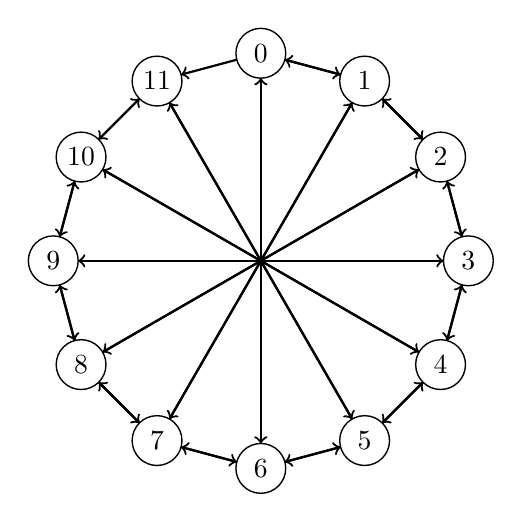
\begin{tikzpicture}[scale=0.50]

\Vertex[x=187.5pt,y=337.5pt]{0};
\Vertex[x=262.5pt,y=317.4038105676658pt]{1};
\Vertex[x=317.4038105676658pt,y=262.5pt]{2};
\Vertex[x=337.5pt,y=187.5pt]{3};
\Vertex[x=317.4038105676658pt,y=112.50000000000004pt]{4};
\Vertex[x=262.5pt,y=57.596189432334185pt]{5};
\Vertex[x=187.50000000000003pt,y=37.5pt]{6};
\Vertex[x=112.50000000000004pt,y=57.596189432334185pt]{7};
\Vertex[x=57.59618943233425pt,y=112.49999999999991pt]{8};
\Vertex[x=37.5pt,y=187.49999999999997pt]{9};
\Vertex[x=57.59618943233421pt,y=262.5pt]{10};
\Vertex[x=112.49999999999994pt,y=317.4038105676658pt]{11};

\tikzset{EdgeStyle/.style={->}}

\Edge(0)(1)
\Edge(1)(2)
\Edge(2)(3)
\Edge(3)(4)
\Edge(4)(5)
\Edge(5)(6)
\Edge(6)(7)
\Edge(7)(8)
\Edge(8)(9)
\Edge(9)(10)
\Edge(10)(11)

\Edge(0)(11)
\Edge(1)(0)
\Edge(2)(1)
\Edge(3)(2)
\Edge(4)(3)
\Edge(5)(4)
\Edge(6)(5)
\Edge(7)(6)
\Edge(8)(7)
\Edge(9)(8)
\Edge(10)(9)
\Edge(11)(10)

\Edge(0)(6)
\Edge(1)(7)
\Edge(2)(8)
\Edge(3)(9)
\Edge(4)(10)
\Edge(5)(11)
\Edge(6)(0)
\Edge(7)(1)
\Edge(8)(2)
\Edge(9)(3)
\Edge(10)(4)
\Edge(11)(5)

\end{tikzpicture}
\caption{ $\Cay(\Z_{12}, \{1, 6, 11\})$.}
\end{center}
\end{figure}
Note that $\Cay(\Z_{12}, \{1, 6, 11\})$ has the same diameter and degree as the $3$-cube, but this graph contains $12$ vertices.  It is natural to ask for the maximum number of vertices a Cayley digraph could possibly have with given diameter and maximum degree.  Cayley digraphs $\Cay(\Z_{m},\mathscr A)$ of $\Z_{m}$ are called $\emph{circulant}$ (di)graphs.  In this paper, we focus on circulant graphs.  However, $n$-cubes may not be as efficient as circulant graphs of equal degree and diameter.  Cayley digraphs, and circulant graphs in particular are often used as models for interconnection networks. As such, it is naturally desirable to maximize the number of vertices which can be connected with constraints on diameter and degree.
For any positive integer $d$ we define
\[
m(d,\mathscr{A}) =\max\{m \vert \diam(Cay(m,\mathscr{A})) \leq d\},
\]
the largest positive integer $m$ such that the diameter, $d(m,\mathscr{A})$, of the Cayley digraph $\Cay(m,\mathscr{A})$ is less than or equal to $d$. For positive integers $d$ and $k$,
\[
m(d,k) = \max\{m(d,\mathscr{A}) \vert \vert \mathscr{A} \vert = k \},
\]
the maximum modulus m such that there exists a generating set with cardinality equal to $k$ and the diameter of the Cayley digraph is less than or equal to $d$. 
$\\$

It is clear that $m(1,k) = k+1$ and $m(d,1) = d+1$.
In 1974 Wong and Coppersmith \cite{Wong-Coppersmith:1974} proved that, for positive integers $d$ and $k$,
\[
\left \lfloor \frac dk + 1 \right \rfloor^k \leq m(d, k) \leq  \binom{k + d}k . 
\]
To see the the upper bound, let $|\mathscr{A}| = k$ such that $\diam(Cay(\Z_m, \mathscr{A})) \leq d$. Noting that every element in $\Z_m$ is the sum of at most $d$ not necessarily distinct elements of $\mathscr{A}$, and the commutativity of integers,  we see that
\[
m \leq \binom{k + 1 + d - 1}k = \binom{k + d}k,
\] 
thus proving the upper bound.
Let
\[t = \left \lfloor \frac{d}{k} \right \rfloor + 1\]
and 
\[\mathscr{A} = \{1, t, t^2, ... , t^{k-1}\}.\]
For any $x \in [0, t^k -1]$ we have
\[x = \sum_{i=1}^{k - 1}c_it^i.\]
Since 
\[
\sum_{i=1}^{k} c_i \leq k(t - 1) = k \left \lfloor \frac dk \right \rfloor  \leq d,
\]
we see that $d(0, x) \leq d$. Hence, $\diam(Cay(\Z_{t^k}, \mathscr{A}) \leq d$. Thus we see
\[m(d, k) \geq t^k  = \left \lfloor \frac dk + 1 \right \rfloor^k.
\]

Hsu and Jia \cite{JiaHsu} proved that 
\begin{equation}\label{eqn:m(d,2)>27}
m(d,2) =\left \lfloor \frac{d(d+4)}{3}\right \rfloor+1
\end{equation}
for all $d\geq2$.
 
We will begin by examining the case when k = 3. The current bounds for this case, as $d\to\infty$, are
\[
\frac{176}{2197}d^3 + O(d^2) \leq m(d,3) \leq \frac{1}{14-3\sqrt{3}}(d+3)^3 .
\]
 




\section{The Algorithm}

We now provide an algorithm that takes as an input a set of generators as well as two other permutation sets. These inputs are used to test the ability of a generated lower bound to provide a set covering for our Cayley Graph. The algorithm iterates through permutations of the generating set and possible coverings, giving as an output the maximal generating set as well as the optimal polynomial bound.\\

Let $d$ be the diameter for $\Cay(m, k)$.\\

Given $d$ define $d_{1}$ fixed to be $\frac{d}{\lambda}$, also define $a_{1} = \frac{a}{\lambda}$, $b_{1} = \frac{b}{\lambda}$, and $c_{1} = \frac{c}{\lambda b}$, etc.., so $\lambda$ is a large number determined by $d$. The parameter $\lambda$ will not appear in the code, but it enables us to compute a lower bound as a function of $d$.\\

Our lower bound on $m(d, k)$ will be defined as $m =\alpha \lambda a_{1} + \beta \lambda b_{1} + \gamma \lambda c_{1}$+ ... $\psi \lambda z_{1}$.  To determine the validity of the lower bound, we compute every point in $dA$ as a polynomial in terms of $\lambda$.\\

$\forall$ ($x_{1}, x_{2}, ... , x_{n}$) such that $x_{1} \leq b_{1}, x_{2} \leq c_{1}, .. , x_{n} \leq \psi$ and $\sum_{i} x_{i} \leq d$ define polynomials that are considered to be (new term needed here).\\

$\forall$ constructed lower bounds $x = x_{1}a + x_{2}b + .. + x_{n}k$, we remove dependent linear combinations by comparing the coefficients $(x_{1}, x_{2}, x_{3}, .. , x_{n})$ and $(\alpha, \beta, \gamma, .. , \psi)$ from their respective polynomials.\\

The constructed lower bounds are defined to be regular if $x \in \mathbb{Z}_{m}$. In this way we are able to check $dA \cong to \mathbb{ZZ}_{m}$ by only considering a single representative of $\mathbb{Z}_{m}$.
\\ Note that a regular polynomial need not be minimal.\\

$\forall x \in dA$ if $x \notin Z_m$, we can identify $x$ with point $x' = (x'_{1}, x'_{2}, .. , x'_{k}) \in \mathbb{Z}_{m}$ congruent to $x$ $(mod$ $m)$.  Then if every point $n \in \mathbb{Z}_{m}$ is either equal to some $x$ or $x'$, $dA = \mathbb{Z}_m$. \\

Consider the case, $x > m(d, k)$, where $x$ is not regular. We perform a recursive polynomial subtraction of the coefficients where $\alpha, \beta, \gamma, ... , \psi$ is subtracted term-by-term from $x_{1}, x{2}, x{3}, ... , x{n}$. The resulting low-order coefficients are then forced to be positive by adding the generator associated with the next higher-order term.\\

For example, a resulting polynomial that has been forced to be well formed may look as, $[\lambda(x_{1} - 2 \alpha) + 1]a_{1} + [\lambda(x_{2} - 2 \beta) + 2]b_{1} + [\lambda(x_{3} - 2 \gamma]c_{1} + ... + [\lambda(x_{n} - 2 \psi]z_{1}]$.\\

To construct a lower bound, we systematically check combinations of generators $A$ and coefficients, and record the largest $m$ (and corresponding generators) such that a covering by $dA$ is achieved.

\subsection{Pseudocode}

\begin{algorithmic}

\ForAll{$X = (ax_{1} + bx_{2} + cx_{3} + .. + zx_{n}), M = (\alpha a + \beta b + \gamma c + .. + \psi z)$}  
\State X - M
\EndFor
\end{algorithmic}

\pagebreak



\section{A New Lower Bound for $m(2,k)$}
Let $d$ and $k$ be  positive integers. Let $n(d, k)$ denote the largest positive integer $n$ such that there exists a subset $\mathscr{A}$ of $k$ positive integers with the property that every integer in the interval $[0, n]$ is the sum of at most $d$ not necessarily distinct elements of $\mathscr{A}$. In other words, 
\[
n(d, k) = \max_{\scriptstyle \mathscr{A}\subseteq\mathbb Z^{+}\atop\scriptstyle |\mathscr{A}|=k}\{n\  |\ d \mathscr{A}\supseteq[0, n]\}.
\]
Recall that $d\mathscr A$ denotes the set of all sums of at most $d$ not necessarily distinct elements of $\mathscr A$. The computation of  $n(d, k)$ is often referred as the \emph{postage stamp problem}. The postage stamp problem is an old problem in number theory that has been studied extensively. See \cite{Hsu-Jia:CombinatorialNetworks,Selmer:1986a,Selmer:1986b} for more information. 
A simple construction shows that 
\[
n(2,k)\ge \frac14k^{2}+O(k).
\]
 Rohrbach \cite{Rohrbach:1937a} conjectured in 1937 that
\begin{equation}\label{eqn:Rohrbach's.conjecture.on.n_{alpha}(2,k)}
n(2,k)\sim\frac14{k^2},
\end{equation}
H\"ammerer and Hofmeister \cite{Hammerer-Hofmeister:1976} proved in
1976 by an explicit construction
of a $2$-basis that
\[
n(2,k)\ge \frac {5}{18}{k^2}+O(k),
\]
which disproves the conjecture of Rohrbach
(\ref{eqn:Rohrbach's.conjecture.on.n_{alpha}(2,k)}).
The  best known lower bound for $n(2,k)$ was proved by Mrose \cite{Mrose1979}
\begin{equation}\label{eqn:n(2k)}
n(2, k) \geq \frac{2}{7}k^2 + \frac{12}{7}k + O(1)\qquad  \text{as}\quad  k \to \infty.
\end{equation}
If  $d\mathscr{A}\supseteq[0, n]$ then  $d\mathscr{A}=\Z_{n+1}$. Therefore, for all positive integers $d$ and $k$ we have 
\[
m(d, k) \geq n(d, k)+1.
\]
This implies the best known lower bound for $m(2,k)$ in (\ref{eqn:m(d,2)>27}) before our result in this paper.
 Our proof uses a similar construction to one used by Torleiv Klove and Mossige used to prove the above lower bound on $n(2,k)$ in (\ref{eqn:n(2k)}).  We used a computer program to test candidates for the values that appeared in the proof as the subscripts $\mu,\ \nu$ and $\eta$.  It is likely that our result could be improved upon by a more complicated construction using a larger number of the same types of subsets.  However, testing larger constructions becomes computationally difficult, and there is a theoretical limit of $1/3$ on the leading coefficient of such a construction.  Any lower bound better than $\displaystyle\frac13k^2 + O(k)$ would be of interest.
\begin{theorem}\label{thm:m(2k)}
$\displaystyle m(2,k) \geq \frac{37}{121}k^2 + O(k)$  as $ k \to \infty$.
\end{theorem}
et $k \geq$ 14 be an integer. Let $\displaystyle k_1 = \left \lfloor \frac{k - 3}{11} \right \rfloor$. Let $m = 37k_1^2$.  Define 
\begin{align*}
I_\mu &= [\mu k_1^2, \mu k_1^2 + k_1],
&&\mu = 0, 4, 15, 26; \\
S_\nu &= \{\nu k_1^2 + ik_1 \ |\  i = 0 , 1, ... , k_1 - 1\},
&&\nu = 0, 1, 2, 3;\\
T_{\eta} &= \{\eta k_1^2+ i(k_1 + 1) \ |\   i = 0 , 1, ... , k_1 -1\},
&&\eta = 10, 20, 30.
\end{align*}
 Let $S= S_{0} \cup S_{1} \cup S_{2} \cup S_{3}$, and
define
\[
\mathscr{A}=I_0\cup I_4\cup I_{15}\cup I_{26}\cup S\cup T_{10}\cup T_{20}\cup T_{30}.
\]
Noting  that $I_0\cap S_0=\{0\}$, and 
\[
|I_\mu| = k_1 + 1,\quad 
|S_\nu| = k_1,\quad\text{and}\quad
|T_\eta| = k_1,
\]
we see that 
\[
|\mathscr{A|} \leq 11k_1 + 3 \leq k.
\]  
We now prove that $\mathscr{A}+\mathscr{A}=\Z_m$.
We begin by claiming $I_{\mu}+T_{\eta}\supseteq[(\mu + \eta )k_1^2 ,  (\mu + \eta  + 1)k_1^2)$. Let $n \in[(\mu + \eta )k_1^2 ,  (\mu + \eta  + 1)k_1^2)$.
Then we can write $n$ as 
\[
n = (\mu + \eta ) k_1^2 + qk_1 + r,
\]
where $0 \leq q < k_1$ and $0 \leq r < k_1$.

If $r \geq q$, then $0\le r-q<k_{1}$ and
\[
n = \mu k_1^2 +  (r - q)+ \eta k_1^2 + q(k_1+1).
\]
 Since 
 \[
 \mu k_1^2 + (r - q) \in I_\mu\qquad\text{and}\qquad \eta k_1^2 +q(k_1+1) \in T_\eta,
 \]
we see that $n \in I_{\mu}+T_{\eta}$. 

If $r < q$, then we must have $q \geq 1$ and $0\le k_{1}+r-q+1\le k_{1}$. Then
\[
\mu k_1^2 + (k_1 + r - q + 1) \in I_\mu \qquad \text{and}\qquad
\eta k_1^2 + (q - 1)(k_1 + 1) \in T_\eta.
\]
 Hence
\[
n = \mu k_1^2 + (k_1 + r - q + 1)+\eta k_1^2 + (q - 1)(k_1 + 1) \in I_{\mu}+T_{\eta}.
\]
 

Next we claim that  $I_{\mu}+S_{\nu}\supseteq[(\mu + \nu )k_1^2 ,  (\mu + \nu  + 1)k_1^2)$. Let $n \in[(\mu + \nu )k_1^2 ,  (\mu + \nu  + 1)k_1^2)$.
Then we can write $n$ as 
\[
n = (\mu + \nu ) k_1^2 + qk_1 + r = \mu k_1^2 + r+\nu k_1^2 + qk_1,
\]
where  $0 \leq q < k_1$ and $0 \leq r < k_1$, such that 
\[
\mu k_1^2 + r \in I_\mu \qquad\text{and}\qquad\nu k_1^2 + qk_1 \in S_\nu,
\]
 so $n \in I_{\mu}+S_{\nu}$. 

Our final claim is $S+T_\eta \supseteq[(\eta  +1)k_1^2 ,  (\eta  + 4)k_1^2)$.  Let $n \in[(\eta  +1)k_1^2 ,  (\eta  + 4)k_1^2)$.
Then we can write $n$ as 
\[
n = (\eta  + \nu ) k_1^2 + qk_1 + r, 
\]
where $1 \leq \nu  \leq 3$, $0 \leq q < k_1$, and $0 \leq r < k_1$. 

If $q \geq r$, then
\[
n = \nu k_1^2 + (q - r) k_1+\eta k_1^2 + r(k_1 + 1), 
\]
where $\nu k_1^2 + (q - r)k_1 \in S_\nu$ and $\eta k_1^2 + d(k_1 + 1) \in T_\eta$, so $n \in S_\nu +T_\eta$. 

If $q <r$, then
\[
n = (\nu  - 1)k_1^2 + (k_1 + q - r) k_1+\eta k_1^2 + r(k_1 + 1), 
\]
where 
\[
(\nu  - 1)k_1^2 + (k_1 + q - r)k_1 \in S_{\nu  - 1}\qquad\text{and}\qquad
\eta k_1^2 + r(k_1 + 1) \in T_\eta.
\]
Hence $n \in S_{\nu-1}+T_\eta\subseteq S+T_{\eta}$. 
It is clear that, in $\Z_{37k_{1}^{2}}$,
\begin{align*}
[45k_{1}^{2},46k_{1}^{2})&=[8k_1^2, 9k_1^2),\\
[46k_{1}^{2},47k_{1}^{2})&=[9k_1^2, 10k_1^2),\\
[56k_{1}^{2},57k_{1}^{2})&=[19k_1^2, 20k_1^2).
\end{align*}
Therefore, we have proved that the entire interval $[0, m)=\Z_{m}$ can be  {\em covered\/} as follows: 
\begin{align*}
I_0 + S  &\supseteq [0, 4k_1^2),\\
I_4 + S  &\supseteq [4k_1^2, 8k_1^2),\\
I_{15} + T_{30}  &\supseteq[45k_{1}^{2},46k_{1}^{2})= [8k_1^2, 9k_1^2),\\
I_{26} + T_{20}  &\supseteq[46k_{1}^{2},47k_{1}^{2})= [9k_1^2, 10k_1^2),\\
I_{0}+T_{10}  &\supseteq [10k_1^2, 11k_1^2),\\
S+T_{10}  &\supseteq [11k_1^2, 14k_1^2),\\
I_{4} + T_{10}  &\supseteq [14k_1^2, 15k_1^2),\\
I_{15} + S  &\supseteq [15k_1^2, 19k_1^2),\\
I_{26} + T_{30}  &\supseteq[56k_{1}^{2},57k_{1}^{2})= [19k_1^2, 20k_1^2),\\
I_{0} + T_{20}  &\supseteq [20k_1^2, 21k_1^2),\\
S + T_{20}  &\supseteq [21k_1^2, 24k_1^2),\\
I_{4} + T_{20}  &\supseteq [24k_1^2, 25k_1^2),
\end{align*}
\begin{align*}
I_{15} + T_{10}  &\supseteq [25k_1^2, 26k_1^2),\\
I_{26} + S  &\supseteq [26k_1^2, 30k_1^2),\\
I_{0} + T_{30}  &\supseteq [30k_1^2, 31k_1^2),\\
S + T_{30}  &\supseteq [31k_1^2, 34k_1^2),\\
I_{4} + T_{30}  &\supseteq [34k_1^2, 35k_1^2),\\
I_{15} + T_{20}  &\supseteq [35k_1^2, 36k_1^2),\\
I_{26} + T_{10}  &\supseteq [36k_1^2, 37k_1^2).\qquad\qquad\qquad\ 
\end{align*}
It now follows that 
\[
\mathscr{A} + \mathscr{A} \supseteq [0, 37k_1^2).
\]
Hence
\begin{align*}
m(2,k) &\geq 37k_1^2\\
&= 37 \cdot \left \lfloor \frac{k - 2}{11}\right \rfloor^2\\
&> 37 \left(\frac{k - 2}{11} -1\right) ^2\\
&= \frac{37}{121}k^2-\frac{962}{121}k+\frac{6253}{121}\\
&= \frac{37}{121}k^2 + O(k)\qquad \text{ as }\quad k \to \infty. 
\end{align*}
Theorem~\ref{thm:m(2k)} is proved.

\section{Extension to the General Case}
\begin{theorem}\label{thm:m(dk)}
For any integer $d \geq 2$, as $k \to \infty$, we have 
\[
m(d,k) \geq \left(\frac{148}{121}\right)^{\lfloor \frac{d}{2}\rfloor}\left(\frac{k}{d}\right)^d + O(k^{d-1}).
\]
\end{theorem}
Before we start the proof of Theorem~\ref{thm:m(dk)}, we state and prove the following addition lemma for $m(d,k)$. 
\begin{lemma}\label{lemma:addition}
Given positive integers $k_{1}$, $k_{2}$, $d_{1}\ge2$ and $d_{2}\ge 2$, we have
\[
m(d_1+d_2,k_1+k_2) \geq m(d_1,k_1)m(d_2,k_2) 
\]
\end{lemma}
\begin{proof}[Proof of Lemma~\ref{lem:addition}]
Let $\mathscr{A}_1$ and $\mathscr{A}_2$ be sets of positive integers such that $m(d_1,\mathscr{A}_1) = m(d_1,k_1)$ and $m(d_2,\mathscr{A}_2) = m(d_2,k_2)$.  Since $d_1, d_2 \geq 2$ we have that $m(d_1,k_1)$ is greater than every element in $\mathscr{A}_1$, and similarly for $m(d_2,k_2)$ and $\mathscr{A}_2$.  So let $\mathscr{A} = \mathscr{A}_1 \cup \{m(d_1,k_1)\cdot x \quad \vert \quad x \in \mathscr{A}_2\}$.  Then it suffices to show that $\mathscr{A}$ is a $(d_1+d_2)$-basis for $\mathbb{Z}_{m(d_1,k_1)m(d_2,k_2)}$.  We do this by writing $n \in \mathbb{Z}_{m(d_1,k_1)m(d_2,k_2)}$ as $xm(d_1,k_1) + r$ where $x \in \mathbb{Z}_{m(d_2,k_2)}$ and $r \in \mathbb{Z}_{m(d_1,k_1)}$.  Then $xm(d_1,k_1) \in d_1\mathscr{A}_1\{m(d_1,k_1)\cdot x \quad \vert \quad x \in \mathscr{A}_2\}$ and $r \in d_2\mathscr{A}_1$, so $n \in (d_1+d_2)\mathscr{A}$.
\end{proof}
\begin{proof}[Proof of Theorem~\ref{thm:m(dk)}]
Let $d = 2q +r$ where $q =\displaystyle\left \lfloor \frac{d}{2}\right\rfloor$ and $k = du +v$ where $u =\displaystyle \left \lfloor \frac{k}{d}\right\rfloor$. We separate the calculation into two cases.
Case 1: If $r = 0$, then
\begin{align*}
m(d,k) &= m(2q, du +v)\\
&= m(2q, (2q)u +v)\\
&\geq m(2q, 2qu) \geq m(2, 2u)^q\\
&\geq \left(\frac{37}{121}(2u)^2+ O(u)\right)^q \\
&= \left(\frac{148}{121} \left(\frac{k-v}{d}\right) ^2+ O(u)\right)^{ \frac{d}{2}}\\
&= \left(\frac{148}{121}\right)^{ \frac{d}{2}}\left(\frac{k}{d}\right)^d + O(k^{d-1})
\end{align*}

Case 2: If $r = 1$, then
\begin{align*}
m(d,k) &= m(2q+1, du +v)\\
&= m(2q+1, (2q+1)u +v)\\
&\geq m(2q+1, 2qu + u) \geq m(2, 2u)^q \cdot m(1,u)\\
&\geq \left(\frac{37}{121}(2u)^2+ O(u)\right)^q \cdot (u+1) \\
&= \left(\frac{148}{121} u^2 + O(u)\right)^{ \frac{d-1}{2}} \cdot (u+1)\\
&= \left(\frac{148}{121}^{ \frac{d-1}{2}} u ^{d-1}+ O(u^{d-2})\right) \cdot (u+1)\\
&= \frac{148}{121}^{ \frac{d-1}{2}} u ^{d}+ O(u^{d-1})\\
&= \left(\frac{148}{121}\right)^{ \frac{d-1}{2}}\left(\frac{k}{d}\right)^d + O(k^{d-1})
\end{align*}
Hence 
\[
m(d,k) \geq \left(\frac{148}{121}\right)^{\lfloor \frac{d}{2}\rfloor}\left(\frac{k}{d}\right)^d + O(k^{d-1}).
\]
The proof of Theorem~\ref{thm:m(dk)} is complete.
\end{proof}


\section{ New Lower Bound of $m(d, 4)$.}
Wong and Coppersmith proved that
\[m(d, k) \geq \left (\frac{d}{k} + 1\right)^k.\]
Jia proved that 
\[ 
m(d, 4) \geq2.048 \left(\frac{d}{4}\right)^4  +O(d^3)\qquad\text{as}\quad d\to\infty.
\]
This is currently the best known lower bound for $m(d, 4)$. 

In this paper we will show that \[m(d,4) \geq \frac{512}{243}\left(\frac d4\right)^4 + O(d^3)\approx 2.106996 \left(\frac d4\right)^4 + O(d^3)\].
\begin{theorem} As $d\to\infty$, 
\[
m(d,4) \geq \frac{512}{243}\left(\frac d4\right)^4 + O(d^3)\approx 2.106996 \left(\frac d4\right)^4 + O(d^3).
\]
\end{theorem}

\begin{proof}
Let $d \geq 11$ be an integer and let $\lambda = \left \lfloor \frac{d - 2}{9} \right \rfloor$. Define
\begin{align*}
\alpha &= 3 \lambda,\\
\beta &=3 \lambda \alpha,\\
\gamma &= 3 \lambda \beta,\\
m &= 2 \lambda \gamma + \lambda \beta + \lambda \alpha + \lambda.
\end{align*}
Let $A = \{1, \alpha, \beta, \gamma\}$. Then
\begin{align*}
m &= 2 \lambda d + \lambda c + \lambda b + \lambda \\
&= 54\lambda^4 + 9\lambda^3 + 3\lambda^2 + \lambda\\
&= \frac{512}{243}\left(\frac d4\right)^4 + O(d^3).
\end{align*}

Let $dA$ denote the set of all sums of at most d not necessarily distinct elements of a generating set $A$ of $\Z_m$. Then for this proof we need to show that $dA = \Z_m$ such that the Cayley digraph Cay$(m, A)$ has diameter $d(m, A) \leq d$. 

Every integer $n$ such that $0 \leq n < m$ can be expressed in the following way:
\[ n = w + x\alpha + y\beta + z\gamma\]
where 
\[ 0 \leq w \leq 3\lambda, \quad 0 \leq x \leq 3\lambda,\quad 0 \leq y \leq 3\lambda,\quad 0 \leq z \leq 2\lambda.\]
Thus we only need to show, for every $0 \leq n < m$, there exists nonnegative integers $\delta_1$, $\delta_2$, $\delta_3$, and $\delta_4$ such that we can write $n$ as
\[ n \equiv \delta_1 + \delta_2 \alpha + \delta_3 \beta + \delta_4 \gamma\]
where 
\[ \delta_1 + \delta_2 + \delta_3 + \delta_4 \leq d.\]

We now consider the following cases:

Case 1.  $0 \leq x_3 < \lambda$. The following subcases need to be considered:\\
Subcase 1.a. If $2 \lambda \leq x_1 < 3 \lambda$ then $0 \leq x_0 < 2\lambda$. \\
If $0 \leq x_1 < 2 \lambda$, we have 
\[ x_0 + x_1 + x_2 + x_3 \leq 3\lambda + 2\lambda + 3\lambda + \lambda = 9\lambda \leq d, \]
which implies that $n = x_0 + x_1\alpha + x_2\beta + x_3\gamma \in dA$. \\
If $2 \lambda \leq x_1 < 3 \lambda$ and  $0 \leq x_0 < 2\lambda$, we have 
\[ x_0 + x_1 + x_2 + x_3 \leq 2\lambda + 3\lambda + 3\lambda + \lambda = 9\lambda \leq d, \]
which implies that $n = x_0 + x_1\alpha + x_2\beta + x_3\gamma \in dA$. 

Subcase 1.b. $2 \lambda \leq x_2 < 3 \lambda$, $2 \lambda \leq x_1 < 3\lambda$, $2 \lambda \leq x_0 < 3\lambda$. \\
We have
\begin{align*}
n \equiv n + m &= x_0 + x_1\alpha + x_2\beta + x_3\gamma + \lambda + \lambda \alpha + \lambda \beta + 2 \lambda \gamma\\
&=  x_0 + \lambda + (x_1 + \lambda) \alpha + (x_2 + \lambda) \beta + (x_3 + 2 \lambda) \gamma\\ 
&=  x_0 -  2\lambda + (x_1 - 2 \lambda + 1) \alpha + (x_2 + \lambda + 1) \beta + (x_3 + 2 \lambda)
 \gamma.\\ 
\end{align*}
Noting that
\[  x_0 -  2\lambda \geq 0, x_1 - 2 \lambda + 1 \geq 0, x_2 + \lambda + 1 \geq 0, \text{ and } x_3 + 2 \lambda \geq 0, \]
we see that 
\begin{align*}
x_0 -  2\lambda + x_1 - 2 \lambda + 1 + x_2 + \lambda + 1 + x_3 + 2 \lambda &= x_0  + x_1 +  x_2 + x_3 -  \lambda + 2 \\
&\leq 3 \lambda + 3 \lambda + 3 \lambda + \lambda - \lambda + 2\\
&= 9 \lambda + 2 \leq d,
\end{align*}
which implies that $n = x_0 + x_1\alpha + x_2\beta + x_3\gamma \in dA$. 

Case 2. $\lambda \leq x_3 < 2\lambda$. The following subcases need to be considered:\\
Subcase 2.a. $0 \leq x_2 < 2 \lambda.$ If $2 \lambda \leq x_1 < 3 \lambda$ then $0 \leq x_0 < 2\lambda$. \\
If $0 \leq x_1 < 2 \lambda$, we have 
\[ x_0 + x_1 + x_2 + x_3 \leq 2\lambda + 2\lambda + 2\lambda + 3\lambda = 9\lambda \leq d, \]
which implies that $n = x_0 + x_1\alpha + x_2\beta + x_3\gamma \in dA$. \\
If $2 \lambda \leq x_1 < 3 \lambda$ and  $0 \leq x_0 < 2\lambda$, we have 
\[ x_0 + x_1 + x_2 + x_3 \leq 2\lambda + 2\lambda + 3\lambda + 2 \lambda = 9\lambda \leq d, \]
which implies that $n = x_0 + x_1\alpha + x_2\beta + x_3\gamma \in dA$. 

Subcase 2.b. $\lambda \leq x_2 < 2 \lambda$, $2 \lambda \leq x_1 < 3\lambda$,  $2\lambda \leq x_0 < 3\lambda$. \\
We have
\begin{align*}
n \equiv n + m &= x_0 + x_1\alpha + x_2\beta + x_3\gamma + \lambda + \lambda \alpha + \lambda \beta + 2 \lambda \gamma\\
&=  x_0 + \lambda + (x_1 + \lambda) \alpha + (x_2 + \lambda) \beta + (x_3 + 2 \lambda) \gamma\\ 
&=  x_0 -  2\lambda + (x_1 - 2 \lambda + 1) \alpha + (x_2 + \lambda + 1) \beta + (x_3 + 2 \lambda)
 \gamma.
\end{align*}
Noting that
\[  x_0 -  2\lambda \geq 0, \  x_1 - 2 \lambda + 1 \geq 0,  \ x_2 + \lambda + 1 \geq 0, \text{ and } x_3 + 2 \lambda \geq 0, \]
we see that 
\begin{align*}
x_0 -  2\lambda + x_1 - 2 \lambda + 1 + x_2 + \lambda + 1 + x_3 + 2 \lambda &= x_0  + x_1 +  x_2 + x_3 -  \lambda + 2 \\
&\leq 3 \lambda + 3 \lambda + 2 \lambda + 2\lambda - \lambda + 2\\
&= 9 \lambda + 2 \leq d,
\end{align*}
which implies that $n = x_0 + x_1\alpha + x_2\beta + x_3\gamma \in dA$. 

Subcase 2.c. $2 \lambda \leq x_2 < 3 \lambda.$ If $ \lambda \leq x_1 < 2 \lambda$ then $0 \leq x_0 < 2\lambda$. \\
If $0 \leq x_1 < \lambda$, we have 
\[ x_0 + x_1 + x_2 + x_3 \leq 3\lambda + \lambda + 3 \lambda + 2\lambda = 9\lambda \leq d, \]
which implies that $n = x_0 + x_1\alpha + x_2\beta + x_3\gamma \in dA$. \\
If $ \lambda \leq x_1 < 2 \lambda$ and  $0 \leq x_0 < 2\lambda$, we have 
\[ x_0 + x_1 + x_2 + x_3 \leq 2\lambda + 2\lambda + 3\lambda + 2 \lambda = 9\lambda \leq d, \]
which implies that $n = x_0 + x_1\alpha + x_2\beta + x_3\gamma \in dA$. 

Subcase 2.d. $2\lambda \leq x_2 < 3 \lambda$, $ \lambda \leq x_1 < 2\lambda$,  $2\lambda \leq x_0 < 3\lambda$. \\
We have
\begin{align*}
n \equiv n + m &= x_0 + x_1\alpha + x_2\beta + x2_3\gamma + \lambda + \lambda \alpha + \lambda \beta + 2 \lambda \gamma\\
&=  x_0 + \lambda + (x_1 + \lambda) \alpha + (x_2 + \lambda) \beta + (x_3 + 2 \lambda) \gamma\\ 
&=  x_0 -  2\lambda + (x_1 + \lambda + 1) \alpha + (x_2 - 2 \lambda) \beta + (x_3 + 2 \lambda + 1)
 \gamma.
\end{align*}
Noting that
\[  x_0 -  2\lambda \geq 0,  \ x_1 + \lambda + 1 \geq 0, \  x_2 - 2 \lambda \geq 0, \text{ and } x_3 + 2 \lambda + 1 \geq 0, \]
we see that 
\begin{align*}
x_0 -  2\lambda + x_1 + \lambda + 1 + x_2  - 2 \lambda + x_3 + 2 \lambda + 1 &= x_0  + x_1 +  x_2 + x_3 -  \lambda + 2 \\
&\leq 3 \lambda + 2 \lambda + 3 \lambda + 2\lambda - \lambda + 2\\
&= 9 \lambda + 2 \leq d,
\end{align*}
which implies that $n = x_0 + x_1\alpha + x_2\beta + x_3\gamma \in dA$. 

Subcase 2.e. $2\lambda \leq x_2 < 3 \lambda$, $ 2\lambda \leq x_1 < 3\lambda$,  $0 \leq x_0 < 2\lambda$. \\
We have
\begin{align*}
n \equiv n + m &= x_0 + x_1\alpha + x_2\beta + x_3\gamma + \lambda + \lambda \alpha + \lambda \beta + 2 \lambda \gamma\\
&=  x_0 + \lambda + (x_1 + \lambda) \alpha + (x_2 + \lambda) \beta + (x_3 + 2 \lambda) \gamma\\ 
&=  x_0 +  \lambda + (x_1 - 2 \lambda) \alpha + (x_2 - 2 \lambda + 1) \beta + (x_3 + 2 \lambda + 1)\gamma.
\end{align*}
Noting that
\[  x_0 +  \lambda \geq 0,  \ x_1 - 2 \lambda \geq 0, \  x_2 - 2 \lambda + 1 \geq 0, \text{ and } x_3 + 2 \lambda + 1 \geq 0, \]
we see that 
\begin{align*}
x_0 + \lambda + x_1 - 2 \lambda + x_2  - 2 \lambda + 1 + x_3 + 2 \lambda + 1 &= x_0  + x_1 +  x_2 + x_3 -  \lambda + 2 \\
&\leq 2 \lambda + 3 \lambda + 3 \lambda + 2\lambda -  \lambda + 2\\
&= 9 \lambda + 2 \leq d,
\end{align*}
which implies that $n = x_0 + x_1\alpha + x_2\beta + x_3\gamma \in dA$. 

Subcase 2.f. $2\lambda \leq x_2 < 3 \lambda$, $ 2\lambda \leq x_1 < 3\lambda$,  $2\lambda \leq x_0 < 3\lambda$. \\
We have
\begin{align*}
n \equiv n + m &= x_0 + x_1\alpha + x_2\beta + x_3\gamma + \lambda + \lambda \alpha + \lambda \beta + 2 \lambda \gamma\\
&=  x_0 + \lambda + (x_1 + \lambda) \alpha + (x_2 + \lambda) \beta + (x_3 + 2 \lambda) \gamma\\ 
&=  x_0 -  2\lambda + (x_1 - 2 \lambda + 1) \alpha + (x_2 - 2 \lambda + 1) \beta + (x_3 + 2 \lambda + 1)\gamma.
\end{align*}
Noting that
\[  x_0 -  2\lambda \geq 0,  \ x_1 - 2 \lambda + 1 \geq 0, \  x_2 - 2 \lambda + 1 \geq 0, \text{ and } x_3 + 2 \lambda + 1 \geq 0, \]
we see that 
\begin{align*}
x_0 -  2\lambda + x_1 - 2 \lambda + 1 + x_2  - 2 \lambda + 1 + x_3 + 2 \lambda + 1 &= x_0  + x_1 +  x_2 + x_3 -  4 \lambda + 3 \\
&\leq 3 \lambda + 3 \lambda + 3 \lambda + 2\lambda - 4 \lambda + 3\\
&= 7 \lambda + 2 \leq d,
\end{align*}
which implies that $n = x_0 + x_1\alpha + x_2\beta + x_3\gamma \in dA$. 

Case 3. $2 \lambda \leq x_3 < 3 \lambda$. The following subcases need to be considered:\\
Subcase 3.a. $0 \leq x_2 <  \lambda.$ If $2 \lambda \leq x_1 < 3 \lambda$ then $0 \leq x_0 < 2\lambda$. \\
If $0 \leq x_1 < 2\lambda$, we have 
\[ x_0 + x_1 + x_2 + x_3 \leq 3 \lambda + 2 \lambda + \lambda + 3\lambda = 9\lambda \leq d, \]
which implies that $n = x_0 + x_1\alpha + x_2\beta + x_3\gamma \in dA$. \\
If $2 \lambda \leq x_1 < 3 \lambda$ and  $0 \leq x_0 < 2\lambda$, we have 
\[ x_0 + x_1 + x_2 + x_3 \leq 2\lambda + 3\lambda + \lambda + 3 \lambda = 9\lambda \leq d, \]
which implies that $n = x_0 + x_1\alpha + x_2\beta + x_3\gamma \in dA$. 

Subcase 3.b. $0 \leq x_2 <  \lambda$, $ 2\lambda \leq x_1 < 3\lambda$,  $2 \lambda \leq x_0 < 3\lambda$. \\
We have
\begin{align*}
n \equiv n + m &= x_0 + x_1\alpha + x_2\beta + x_3\gamma + \lambda + \lambda \alpha + \lambda \beta + 2 \lambda \gamma\\
&=  x_0 + \lambda + (x_1 + \lambda) \alpha + (x_2 + \lambda) \beta + (x_3 + 2 \lambda) \gamma\\ 
&=  x_0 -  2\lambda + (x_1 - 2 \lambda + 1) \alpha + (x_2 + \lambda + 1) \beta + (x_3 + 2 \lambda )\gamma.
\end{align*}
Noting that
\[  x_0 -  2\lambda \geq 0,  \ x_1 - 2 \lambda + 1 \geq 0, \  x_2 + \lambda + 1 \geq 0, \text{ and } x_3 + 2 \lambda \geq 0, \]
we see that 
\begin{align*}
x_0 -  2\lambda + x_1 - 2 \lambda + 1 + x_2  + \lambda + 1 + x_3 + 2 \lambda &= x_0  + x_1 +  x_2 + x_3 -  \lambda + 2 \\
&\leq 3 \lambda + 3 \lambda + \lambda + 3\lambda - \lambda + 2\\
&= 9 \lambda + 2 \leq d,
\end{align*}
which implies that $n = x_0 + x_1\alpha + x_2\beta + x_3\gamma \in dA$.

Subcase 3.c. $\lambda \leq x_2 < 2 \lambda$ and $0 \leq x_1 < 2\lambda$.  If $\lambda \leq x_1 < 2 \lambda$ then $0 \leq x_0 < \lambda$. \\
If $0 \leq x_1 < \lambda$, we have 
\[ x_0 + x_1 + x_2 + x_3 \leq 3\lambda + \lambda + 2\lambda + 3\lambda = 9\lambda \leq d, \]
which implies that $n = x_0 + x_1\alpha + x_2\beta + x_3\gamma \in dA$. \\
If $ \lambda \leq x_1 < 2 \lambda$ and  $0 \leq x_0 < \lambda$, we have 
\[ x_0 + x_1 + x_2 + x_3 \leq \lambda + 2\lambda + 2 \lambda + 3 \lambda = 8\lambda \leq d, \]
which implies that $n = x_0 + x_1\alpha + x_2\beta + x_3\gamma \in dA$.

Thus we have shown that every element $0 \leq n < m$ is contained in $dA$, which implies the diameter of the Cayley digraph Cay$(\Z_m, A)$ is less than or equal to $d$. 
Hence,
\[
m(d, 4) \geq2.048 \left(\frac{d}{4}\right)^4  +O(d^3)\qquad\text{as}\quad d\to\infty. \qedhere
\]
\end{proof}


\input{future}


\section{Open Problems}
\begin{enumerate}[\bf 1.]
\item  Finding a non-trivial lower bound for $m(3,k)$, $m(4,k)$, etc.

\item  For $n(d,k)$ it is known that for every positive integer $k$ the limit 
\[
\lim_{d \to \infty}{\frac{n(d,k)}{d^k}}
\]
exists, and the value is known for $k = 1,$ $2$ and $3$.  It is not known whether or not 
\[
\lim_{d \to \infty}{\frac{m(d,k)}{d^k}}
\]
exists for every k, and the value is only known for $k = 1$ and $2$. \\
\item The limits
\[
\lim_{d \to \infty}{\frac{m(d,k)}{n(d,k)}} \text{ and}
\lim_{k \to \infty}{\frac{m(d,k)}{n(d,k)}}
\]
are also of interest, if they exist.
\item  We may define the undirected version of our extremal function $M(d,k)$ to be the largest $M$ such that there exists of symmetric set $\mathscr{A}$ of $k$ elements and their additive inverses such that $\diam(Cay(\Z_M,\mathscr{A})) \leq d$.  Little is known about $M(d,k)$, for fixed $d$ and $k \geq 3$. \\
\item We may also define the average version of our extremal function $\bar{m}(d,k)$ to be the largest $m$ such that there exists a set $\mathscr{A}$ of $k$ elements such that the average distance between any two vertices in $Cay(\Z_m,\mathscr{A})$ is less than $d$. New lower bounds for $k \geq 3$ would be interesting for this function as well.
\item Although this paper is primarily concerned with lower bounds, upper bounds on $m(d,k)$ (and related functions) are also of interest.

\end{enumerate}


\end {document}
